\begin{figure*}
    \centering
    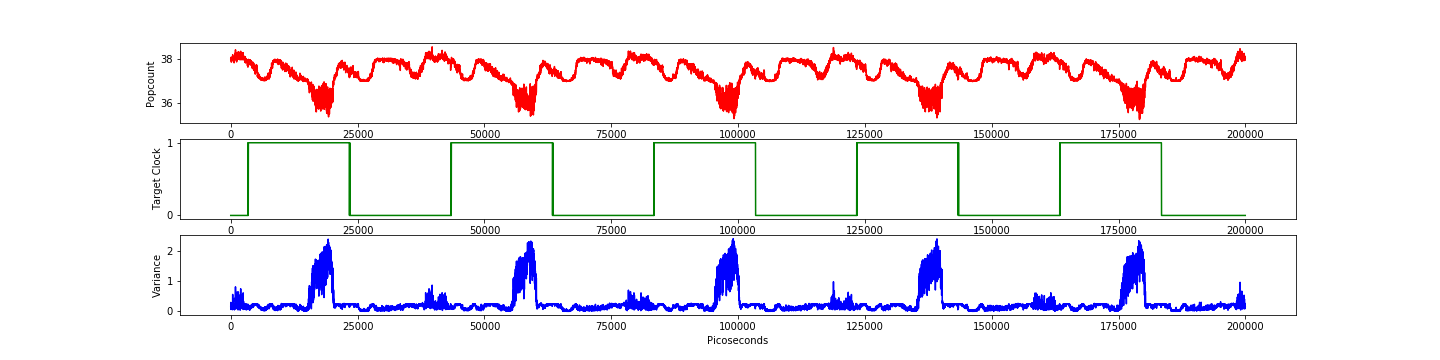
\includegraphics[width=\linewidth]{img/orca_target_25_pop.png}
    \caption{Target clock tuning of the ORCA soft-processor running a common encryption algorithm, AES, at 25MHz. A single trace is gathered at 13440 positions of MMCM \textcircled{1} of Figure \ref{fig:dl-schema}, a phase offset of 200000ps overall. We represent in green where within the 25MHz ORCA clock the positive edge of the 25MHz $F_{sample}$ falls. The average population count (or popcount) in red represents how far on average a positive edge propagates through the carry-chain in a given trace. Within each trace we measure the variability of the popcount, in blue, which shows at what points the sensor has the potential to extract compromising information about a co-tenant. TODO - Green graph is potentially interesting but maybe worth dropping as it is can be confusing at first glance. }
    \label{fig:orca-aes}
\end{figure*}